% Options for packages loaded elsewhere
\PassOptionsToPackage{unicode}{hyperref}
\PassOptionsToPackage{hyphens}{url}
%
\documentclass[
  10pt,
  ignorenonframetext,
  aspectratio=169,t,xcolor=table]{beamer}
\usepackage{pgfpages}
\setbeamertemplate{caption}[numbered]
\setbeamertemplate{caption label separator}{: }
\setbeamercolor{caption name}{fg=normal text.fg}
\beamertemplatenavigationsymbolsempty
% Prevent slide breaks in the middle of a paragraph
\widowpenalties 1 10000
\raggedbottom
\setbeamertemplate{part page}{
  \centering
  \begin{beamercolorbox}[sep=16pt,center]{part title}
    \usebeamerfont{part title}\insertpart\par
  \end{beamercolorbox}
}
\setbeamertemplate{section page}{
  \centering
  \begin{beamercolorbox}[sep=12pt,center]{part title}
    \usebeamerfont{section title}\insertsection\par
  \end{beamercolorbox}
}
\setbeamertemplate{subsection page}{
  \centering
  \begin{beamercolorbox}[sep=8pt,center]{part title}
    \usebeamerfont{subsection title}\insertsubsection\par
  \end{beamercolorbox}
}
\AtBeginPart{
  \frame{\partpage}
}
\AtBeginSection{
  \ifbibliography
  \else
    \frame{\sectionpage}
  \fi
}
\AtBeginSubsection{
  \frame{\subsectionpage}
}
\usepackage{amsmath,amssymb}
\usepackage{iftex}
\ifPDFTeX
  \usepackage[T1]{fontenc}
  \usepackage[utf8]{inputenc}
  \usepackage{textcomp} % provide euro and other symbols
\else % if luatex or xetex
  \usepackage{unicode-math} % this also loads fontspec
  \defaultfontfeatures{Scale=MatchLowercase}
  \defaultfontfeatures[\rmfamily]{Ligatures=TeX,Scale=1}
\fi
\usepackage{lmodern}
\usecolortheme{beaver}
\ifPDFTeX\else
  % xetex/luatex font selection
\fi
% Use upquote if available, for straight quotes in verbatim environments
\IfFileExists{upquote.sty}{\usepackage{upquote}}{}
\IfFileExists{microtype.sty}{% use microtype if available
  \usepackage[]{microtype}
  \UseMicrotypeSet[protrusion]{basicmath} % disable protrusion for tt fonts
}{}
\makeatletter
\@ifundefined{KOMAClassName}{% if non-KOMA class
  \IfFileExists{parskip.sty}{%
    \usepackage{parskip}
  }{% else
    \setlength{\parindent}{0pt}
    \setlength{\parskip}{6pt plus 2pt minus 1pt}}
}{% if KOMA class
  \KOMAoptions{parskip=half}}
\makeatother
\usepackage{xcolor}
\newif\ifbibliography
\setlength{\emergencystretch}{3em} % prevent overfull lines
\providecommand{\tightlist}{%
  \setlength{\itemsep}{0pt}\setlength{\parskip}{0pt}}
\setcounter{secnumdepth}{-\maxdimen} % remove section numbering
%%%%%%%%%%%%%%%%%%%%%%%%%%%%%%%%%%%%%%%%%%%%%%%%%%%%%%%%%%%%%%%%%%%%%%%%%%%%%%%%%%%%%%%
%     <-- выше автоматическая преамбула  |  пользовательская преамбула ниже --->      %
%%%%%%%%%%%%%%%%%%%%%%%%%%%%%%%%%%%%%%%%%%%%%%%%%%%%%%%%%%%%%%%%%%%%%%%%%%%%%%%%%%%%%%%

%%% Работа с русским языком
\usepackage{cmap}					    % поиск в PDF
\usepackage{mathtext} 				% русские буквы в формулах

% Для разметки слайдов и картинок
\usepackage{tikz}
\usepackage{animate}

% Для двойных прямых кавычек в Verbatim (не работает почему-то)
\usepackage{upquote}

% % Работа с прочими шрифтами
% \usepackage{fontspec}      %% УЖЕ ЗАГРУЖЕН В ПРЕАМБУЛЕ подготавливает загрузку шрифтов Open Type, True Type и др.
\setmainfont{Times New Roman} %% задаёт основной шрифт документа
\setsansfont{Microsoft Sans Serif} %% задаёт шрифт без засечек
\setmonofont[Scale=0.7]{DejaVu Sans Mono} %% моноширинный шрифт\

%% математический шрифт
\setmathfont[version=Cambria]    {Cambria Math}
\setmathfont[version=LatinModern]{Latin Modern Math}
\mathversion{Cambria}

% Межстрочный интервал в verabtim
\makeatletter
\def\verbatim@font{\linespread{0.7}\normalfont\ttfamily}
\makeatother

% Межабзацный интервал в columns
\makeatletter
\newcommand{\@minipagerestore}{\setlength{\parskip}{4pt plus 2pt minus 1pt}}
\makeatother

% \usepackage{hyperref} %% УЖЕ ЗАГРУЖЕН В ПРЕАМБУЛЕ
\definecolor{links}{HTML}{2A1B81}
\hypersetup{colorlinks=true,linkcolor=,urlcolor=links,pdfview=FitH,pdfpagelayout=SinglePage, unicode=true,breaklinks=true}

% Тильда в тексте
\newcommand{\mytilde}{\char`~\:}
% argmin и argmax
\DeclareMathOperator*{\argmax}{argmax}
\DeclareMathOperator*{\argmin}{argmin}

% Более простой ввод команд для двухколоночной верстки
\newcommand{\columnsbegin}{\vspace{-0.5\baselineskip}\begin{columns}[t,onlytextwidth]}
\newcommand{\columnsend}{\end{columns}}
\newcommand{\columnbegin}{\begin{column}}
\newcommand{\columnend}{\end{column}}
\newcommand{\blockbegin}{\begin{block}}
\newcommand{\blockend}{\end{block}}

% allows to add alignment keys to \includegraphics
\usepackage[export]{adjustbox}

% Работа с таблицами %%%%%%%%%%%%%%

\usepackage{adjustbox}

% Новые типы колонок для окружения tabular, чтобы можно было задавать их ширину
% Например, \begin{tabular}{ L{2.3cm} C{2cm} C{1.5cm} C{2.5cm} C{4cm}}
\usepackage{array}
\renewcommand{\arraystretch}{1.5}
\newcolumntype{L}[1]{>{\raggedright\let\newline\\\arraybackslash\hspace{0pt}}m{#1}}
\newcolumntype{C}[1]{>{\centering\let\newline\\\arraybackslash\hspace{0pt}}m{#1}}
\newcolumntype{R}[1]{>{\raggedleft\let\newline\\\arraybackslash\hspace{0pt}}m{#1}}

% Для таблиц в tabularx окружении при помощи пакета huxtable
\usepackage{tabularx}

% Прочие настройки beamer %%%%%%%%%%%%

% Цвета
% Посмотреть и конвертировать можно здесь https://convertingcolors.com/
%                       RGB                       HEX    nearest R colour
\definecolor{spbblack}{RGB}{30,30,30}           % 1e1e1e "gray12"
\definecolor{spbgrey}{RGB}{191,191,191}         % BFBFBF "gray75"
\definecolor{spbteal}{RGB}{188, 216, 221}       % BCD8DD "powderblue"
\definecolor{spblightteal}{RGB}{222,236,238}    % DEECEE "azure2"
\definecolor{spbred}{RGB}{203,55,87}            % CB3757 "maroon"
\definecolor{spbgreen}{RGB}{168,207,166}        % A8CFA6 "darkseagreen3"
\definecolor{spbdarkgreen}{RGB}{96,157,131}     % 609D83 "paleturquoise4"
\definecolor{spbblue}{RGB}{98,122,235}          % 627AEB "cornflowerblue"
\definecolor{spbdarkblue}{RGB}{24,112,184}      % 1870B8 "dodgerblue3"
\definecolor{spbviolet}{RGB}{212,207,232}       % D4CFE8
\definecolor{spbdarkviolet}{RGB}{101,118,185}   % 6576B9
\definecolor{spbyellow}{RGB}{254,192,15}        % FEC00F "darkgoldenrod1"
\definecolor{spbsteelblue}{RGB}{70,130,180}     % 4682B4 "steelblue"


% Галочка в тексте
\def\checkmark{\tikz\fill[scale=0.4](0,.35) -- (.25,0) -- (1,.7) -- (.25,.15) -- cycle;}

% Для раскраски таблиц
\usepackage{colortbl}
% переопределяем tabular с раскраской
\let\oldtabular\tabular
\let\endoldtabular\endtabular
\renewenvironment{tabular}{
\setlength\arrayrulewidth{1pt} \arrayrulecolor{white}
\rowcolors{1}{spbteal}{spblightteal}
\oldtabular}{\endoldtabular}

\usepackage{caption}
\captionsetup[table]{name=Таблица}
% переопределяем tabularx с раскраской
\let\oldtabularx\tabularx
\let\endoldtabularx\endtabularx
\renewenvironment{tabularx}{
\setlength\arrayrulewidth{1pt} \arrayrulecolor{white}
\rowcolors{1}{spbteal}{spblightteal}
\oldtabularx}{\endoldtabularx}


% Для подсветки элементов формул
\usepackage[beamer,customcolors,norndcorners]{hf-tikz}
\hfsetfillcolor{spbteal}
\hfsetbordercolor{white}

\setbeamercolor{myfootlinetext}{fg=spbgrey}
\setbeamerfont{myfootlinetext}{size=\normalsize}
% Переопределяем бимеровский footline
\setbeamertemplate{footline}{
  % \vspace{1cm}
  \usebeamercolor[fg]{myfootlinetext}
  \usebeamerfont{myfootlinetext}
  \hspace{0.5cm}\textbf{\insertpagenumber}\hfill\strut\quad
  \vspace{0.4cm}
}

% Фон слайдов
\usepackage{etoolbox}
\makeatletter
\setbeamertemplate{background canvas}{%
   \ifnumequal{\c@framenumber}{1}{%
      % First frame
      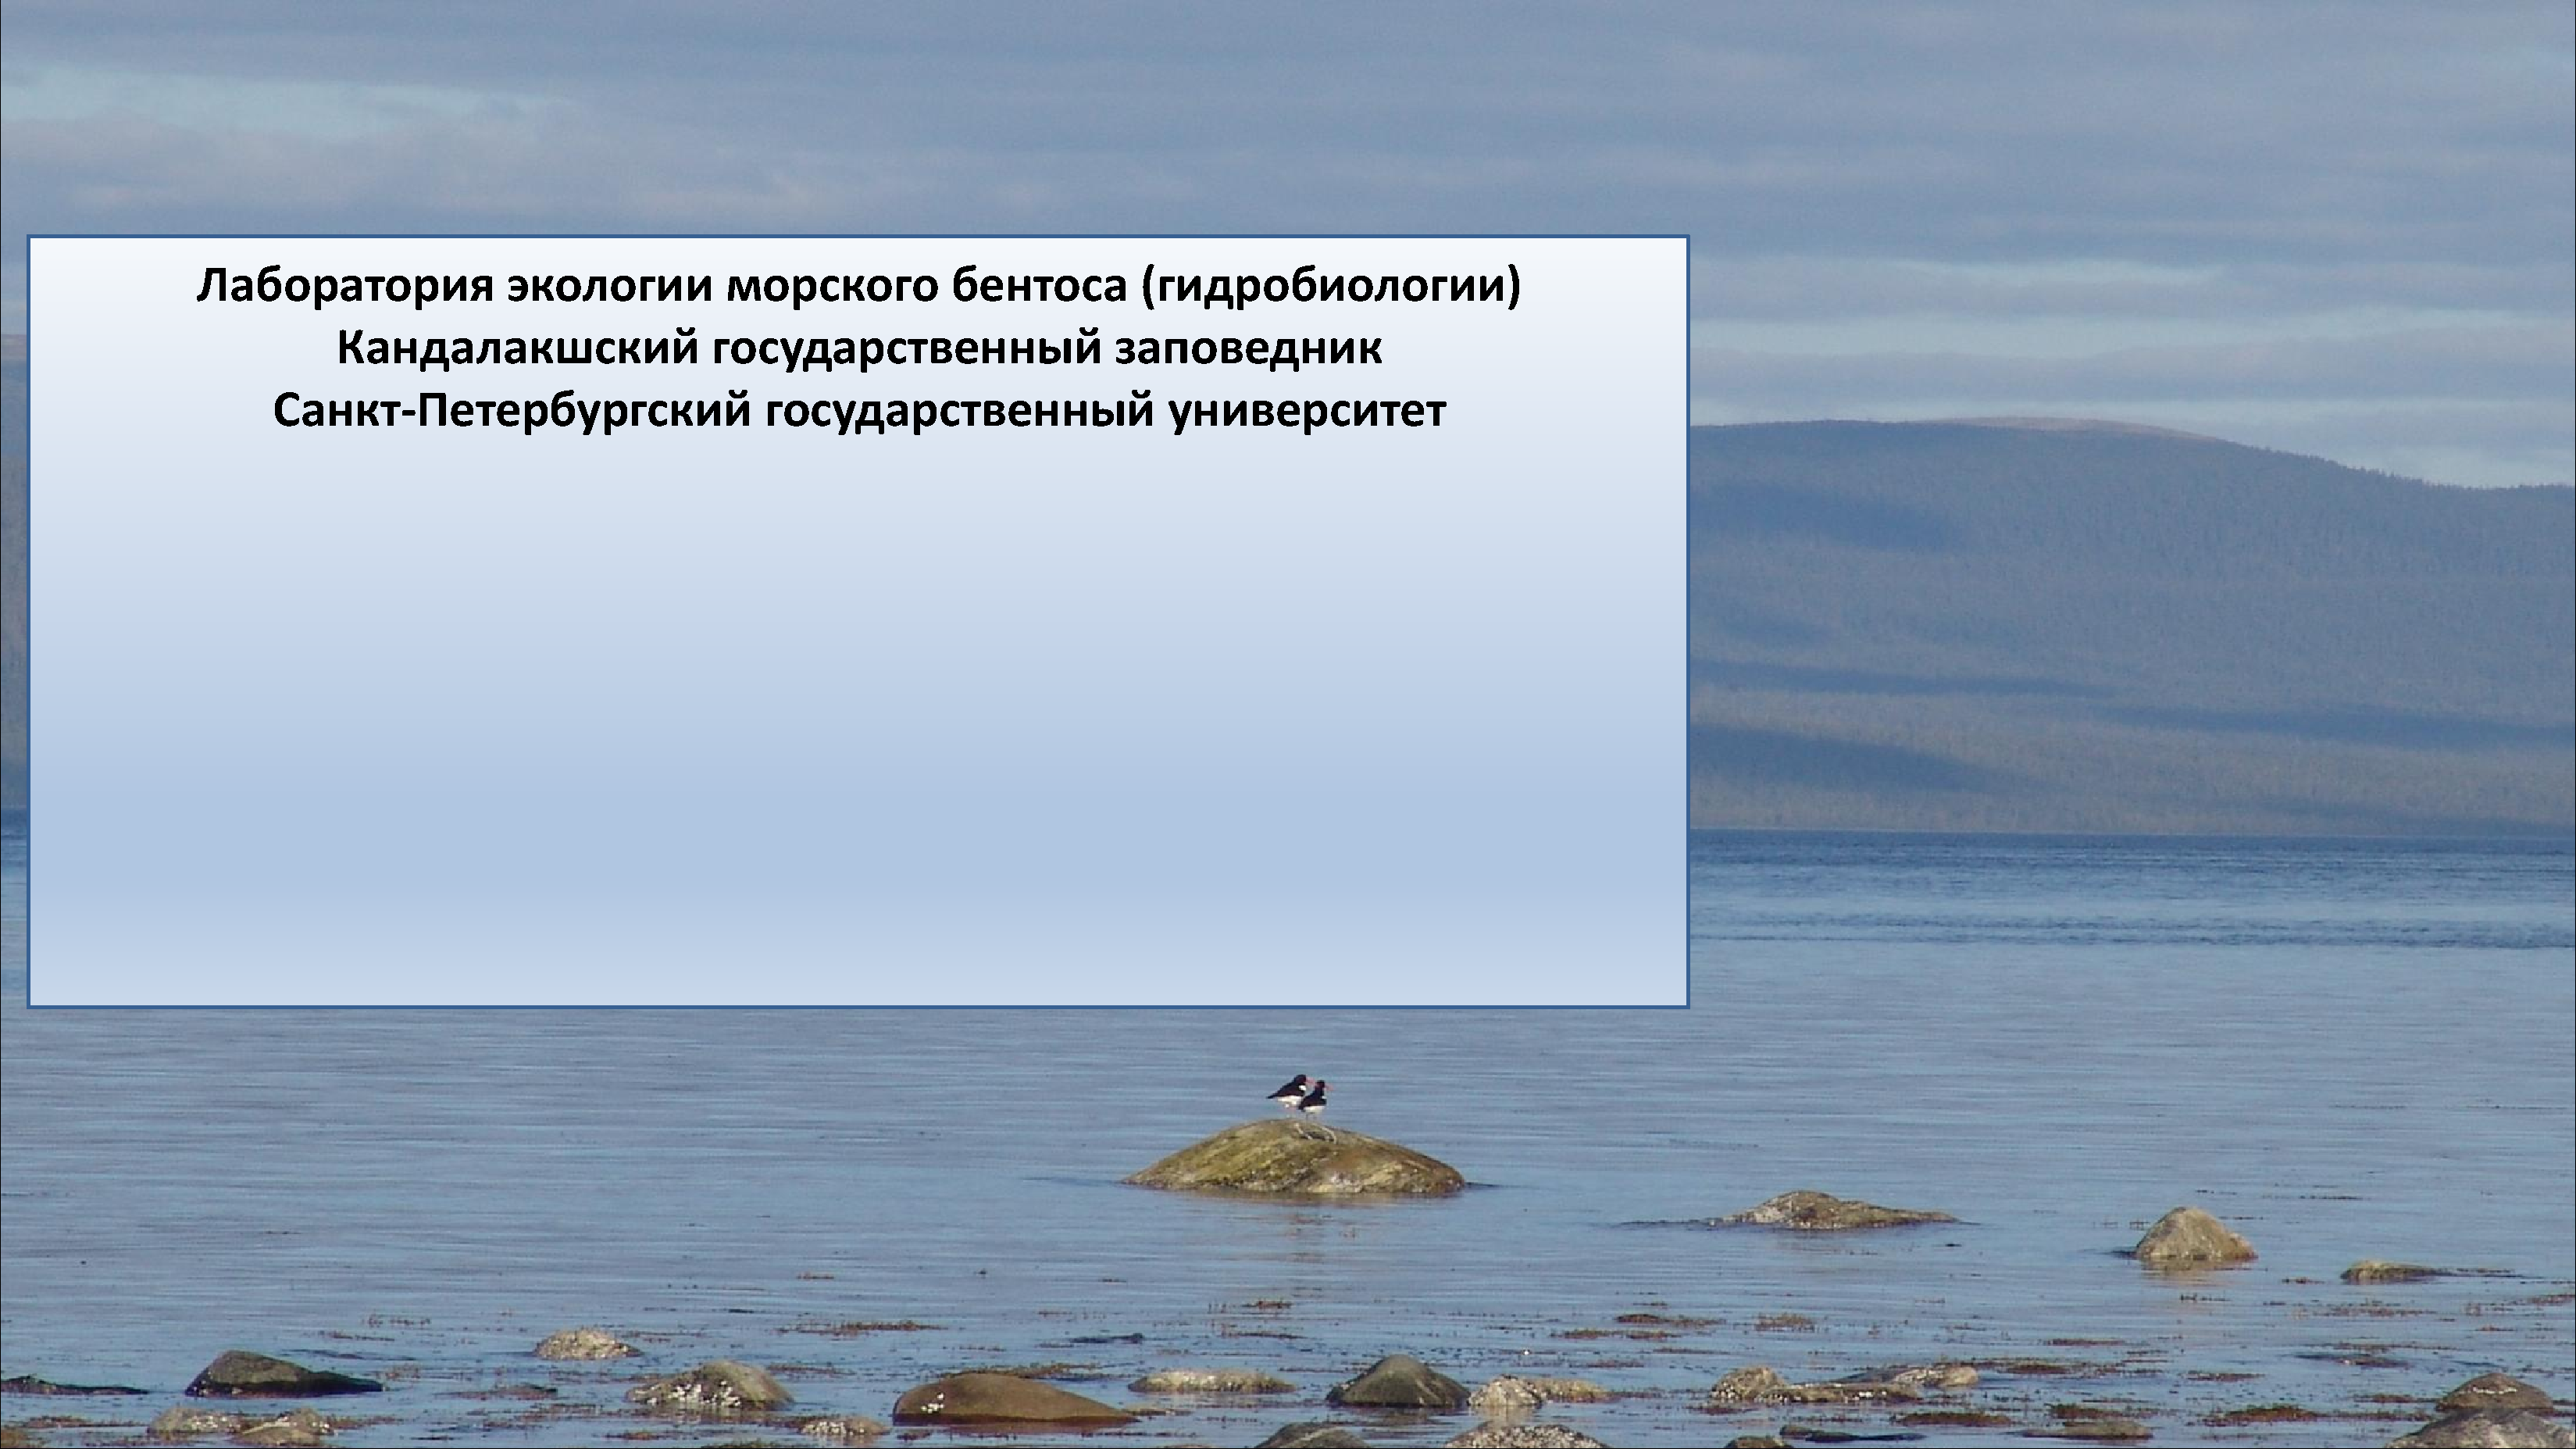
\includegraphics[width=\paperwidth,height=\paperheight]{includes/Primer_title.pdf}
   }{%
      \ifnumequal{\c@framenumber}{\inserttotalframenumber-1}{
         % Before last frame
         
\includegraphics[width=\paperwidth,height=\paperheight]{includes/Primer_sources.pdf}
      }{%
      \ifnumequal{\c@framenumber}{\inserttotalframenumber}{
         % Last frame
         
\includegraphics[width=\paperwidth,height=\paperheight]{includes/Primer_last.pdf}
      }{%
         % Other frames
         
\includegraphics[width=\paperwidth,height=\paperheight]{includes/Primer_slide.pdf}
      }%
   }%
   }%
}
\makeatother

% Разметка титульного слайда
\setbeamertemplate{title page}{%
    \begin{tikzpicture}[remember picture,overlay]
    % Заголовок
    \node[anchor=west]
    at ([yshift=-25mm,xshift=18mm]current page.north west) (title)
    {\parbox[b][1in]{0.45\paperwidth}{\raggedright%
            \usebeamerfont{title}\textcolor{spbblack}{\textbf\inserttitle}}};
    % Автор
    \node[anchor=west]
    at ([yshift=-57mm,xshift=18mm]current page.north west) (author)
    {\parbox[t][1in]{.45\paperwidth}{\raggedright%
            \usebeamerfont{author}\textcolor{spbblack}{\insertauthor}}};
    % Организация
    \node[anchor=north west]
    at ([yshift=37mm,xshift=18mm]current page.south west) (institute)
    {\parbox[t]{.45\paperwidth}{\raggedright%
            \usebeamerfont{institute}\textcolor{spbblack}{\insertinstitute}}};
    \end{tikzpicture}
}
% Заголовок на титульном слайде
\setbeamercolor{titlelike}{parent=palette primary,fg=spbblack,bg=}

% Блоки
\setbeamercolor{block title}{fg=spbblack, bg=}

% Заголовки слайдов
\setbeamercolor{frametitle}{bg=}
\setbeamertemplate{frametitle}{
  \vspace{1cm}
  \color{spbblack}\bfseries\insertframetitle%
}

% Маркеты элементов списка
\setbeamertemplate{itemize items}{\color{spbteal}\normalsize$\bullet$}


%%%%%%%%%%%%%%%%%%%%%%%%%%%%%%%%%%%%%%%%%%%%%%%%%%%%%%%%%%%%%%%%%%%%%%%%%%%%


%     <-- выше пользовательская преамбула | новый Verabtim ниже --->      %
%%%%%%%%%%%%%%%%%%%%%%%%%%%%%%%%%%%%%%%%%%%%%%%%%%%%%%%%%%%%%%%%%%%%%%%%%%%%%%%%%%%%%%%

% Уменьшаем интервалы сверху и снизу Verbatim
% https://stackoverflow.com/a/2319042
\setlength\partopsep{-\topsep}
\addtolength\partopsep{-\parskip}
\addtolength\partopsep{0.9\baselineskip}

% Линия рядом с кодом
\RecustomVerbatimEnvironment{Highlighting}{Verbatim}{
    commandchars=\\\{\},
    frame=leftline,
    framerule=0.75mm,
    rulecolor=\color{spbteal},
    samepage=true,
    baselinestretch=0.8
}

\usepackage{caption}

%%%%%%%%%%%%%%%%%%%%%%%%%%%%%%%%%%%%%%%%%%%%%%%%%%%%%%%%%%%%%%%%%%%%%%%%%%%%

\ifLuaTeX
  \usepackage{selnolig}  % disable illegal ligatures
\fi
\IfFileExists{bookmark.sty}{\usepackage{bookmark}}{\usepackage{hyperref}}
\IfFileExists{xurl.sty}{\usepackage{xurl}}{} % add URL line breaks if available
\urlstyle{same}
\hypersetup{
  hidelinks,
  pdfcreator={LaTeX via pandoc}}

\title{Знакомство с R}
\author{М.А. Варфоломеева, PhD\\
В.М. Хайтов, к.б.н.}
\date{}

\begin{document}
\frame{\titlepage}

\begin{frame}{Опрятные данные (Tidy data)}
\protect\hypertarget{ux43eux43fux440ux44fux442ux43dux44bux435-ux434ux430ux43dux43dux44bux435-tidy-data}{}
В.М. Хайтов, к.б.н.
\end{frame}

\begin{frame}{Исходные данные часто приходится приводить в порядок}
\protect\hypertarget{ux438ux441ux445ux43eux434ux43dux44bux435-ux434ux430ux43dux43dux44bux435-ux447ux430ux441ux442ux43e-ux43fux440ux438ux445ux43eux434ux438ux442ux441ux44f-ux43fux440ux438ux432ux43eux434ux438ux442ux44c-ux432-ux43fux43eux440ux44fux434ux43eux43a}{}
\columnsbegin
\column{0.49\textwidth}


\includegraphics[clip, trim=10mm 0mm 0mm 20mm, width=\textwidth, height=0.7\textheight,keepaspectratio]{images/stock-photo-magic-broom-and-witch-hat-on-a-white-background-731844499.jpg}

\tiny\{\url{https://www.shutterstock.com/image-photo/magic-broom-witch-hat-on-white-731844499}\}

\column{0.49\textwidth}

На подготовку данных к анализу уходит до~80\% времени.

Существуют определенные правила предоставления данных.

Данные, построенные в соответствии с этими требованиями, называются
\textbf{tidy data}, или~\textbf{опрятные данные}.

\columnsend
\end{frame}

\begin{frame}{Проблемы начинаются уже в электронных таблицах}
\protect\hypertarget{ux43fux440ux43eux431ux43bux435ux43cux44b-ux43dux430ux447ux438ux43dux430ux44eux442ux441ux44f-ux443ux436ux435-ux432-ux44dux43bux435ux43aux442ux440ux43eux43dux43dux44bux445-ux442ux430ux431ux43bux438ux446ux430ux445}{}
\columnsbegin

\column{0.49\textwidth}

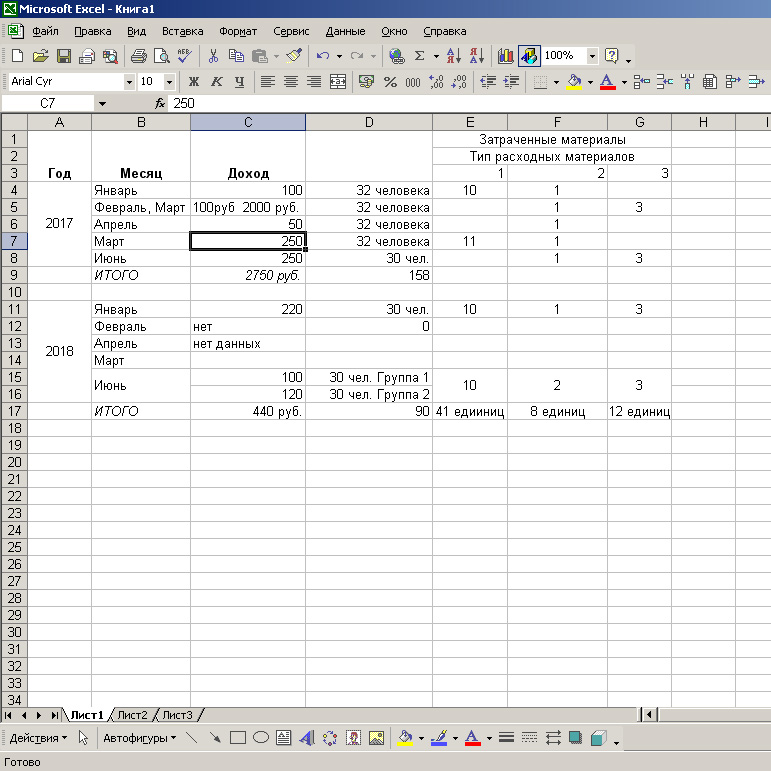
\includegraphics[width=\textwidth, height=0.7\textheight,keepaspectratio]{images/Excel_sheet.jpg}

\column{0.49\textwidth}

\textbf{Основные ошибки}

\begin{itemize}
\tightlist
\item
  Объединенные ячейки
\item
  Отсутствующие заголовки столбцов, вместо них стоят какие-то числа (или
  ничего не стоит) или слишком длинные имена заголовков
\item
  В одной ячейке находится сразу несколько значений
\item
  Разнородные данные в пределах одного столбца
\item
  Нет стандартного обозначения пропущенных значений
\end{itemize}

\columnsend
\end{frame}

\begin{frame}{Tidy data: Основные принципы}
\protect\hypertarget{tidy-data-ux43eux441ux43dux43eux432ux43dux44bux435-ux43fux440ux438ux43dux446ux438ux43fux44b}{}
\begin{itemize}
\tightlist
\item
  Данные (Dataset) --- это набор значений (Values) количественных,
  текстовых, логических.
\item
  Каждое значение принадлежит какой-то переменной (Variable) и какому-то
  наблюдению (Observation).
\item
  При планировании структуры датасета надо помнить, что проще работать с
  колонками, как единым целым, чем со строками. Поэтому удобно, когда в
  таблице столбцы -- переменные, строки -- наблюдения.
\item
  Каждая переменная имеет имя (заголовок столбца).
\end{itemize}
\end{frame}

\begin{frame}[fragile]{Tidy data: Основные принципы}
\protect\hypertarget{tidy-data-ux43eux441ux43dux43eux432ux43dux44bux435-ux43fux440ux438ux43dux446ux438ux43fux44b-1}{}
\begin{itemize}
\tightlist
\item
  Строки (наблюдения) именовать можно, но не обязательно. Если строки
  имеют имя, то оно должно быть уникальным (отличаться от остальных имен
  строк хотя бы номером).
\item
  Каждая переменная содержит только один тип данных.
\item
  Все значения одной переменной измерены в одинаковых единицах
  (например, для всех наблюдений измерения сделаны в сантиметрах).
\item
  Пропущенные значения маркируются единообразно (например, пустые
  ячейки, или \texttt{NA}).
\end{itemize}
\end{frame}

\begin{frame}{Широкий и длинный формат данных}
\protect\hypertarget{ux448ux438ux440ux43eux43aux438ux439-ux438-ux434ux43bux438ux43dux43dux44bux439-ux444ux43eux440ux43cux430ux442-ux434ux430ux43dux43dux44bux445}{}
Одни и те же данные можно представить в широком и длинном формате.

Широкий формат --- каждая строка содержит информацию о нескольких
наблюдениях.

Длинный формат --- каждая строка содержит информацию о единственном
наблюдении.
\end{frame}

\begin{frame}[fragile]{Данные о погибших на ``Титанике'' \newline в
широком и длинном формате}
\protect\hypertarget{ux434ux430ux43dux43dux44bux435-ux43e-ux43fux43eux433ux438ux431ux448ux438ux445-ux43dux430-ux442ux438ux442ux430ux43dux438ux43aux435-ux432-ux448ux438ux440ux43eux43aux43eux43c-ux438-ux434ux43bux438ux43dux43dux43eux43c-ux444ux43eux440ux43cux430ux442ux435}{}
\columnsbegin
\column{0.48\textwidth}

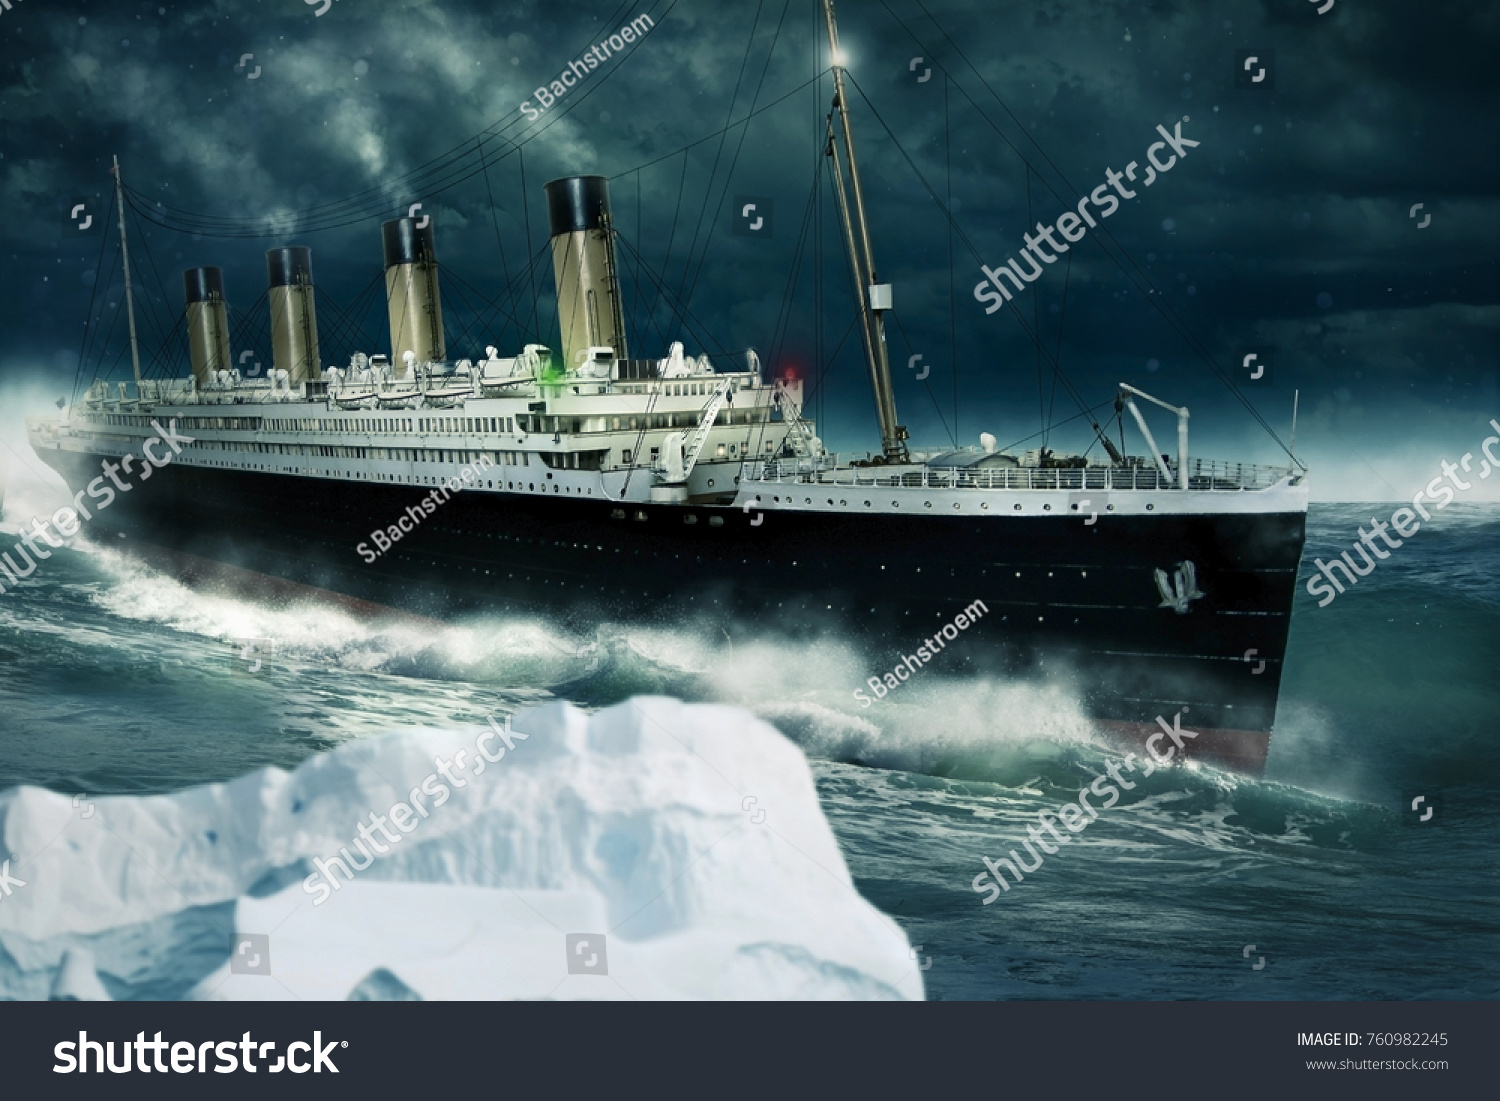
\includegraphics[height=0.6\textheight,keepaspectratio]{./images/stock-photo-old-passenger-ship-rides-over-the-atlantic-760982245.jpg}

\tiny\{\url{https://www.shutterstock.com/ru/image-photo/old-passenger-ship-rides-over-atlantic-760982245}\}

\column{0.48\textwidth}

С представлением данных в широком и длинном формате мы познакомимся на
примере ``Титаника'' (\texttt{Titanic.csv})

\vspace{\baselineskip}

Данные: Dawson, 1995 \newline Источник: пакет \texttt{datasets}

\columnsend
\end{frame}

\begin{frame}[fragile]{Широкий формат данных}
\protect\hypertarget{ux448ux438ux440ux43eux43aux438ux439-ux444ux43eux440ux43cux430ux442-ux434ux430ux43dux43dux44bux445}{}
\columnsbegin
\column{0.49\textwidth}

\begin{verbatim}
#   Class    Sex   Age Survived Freq
# 1   1st   Male Child       No    0
# 2   2nd   Male Child       No    0
# 3   3rd   Male Child       No   35
# 4  Crew   Male Child       No    0
# 5   1st Female Child       No    0
# 6   2nd Female Child       No    0
# 7   3rd Female Child       No   17
# 8  Crew Female Child       No    0
\end{verbatim}

\column{0.49\textwidth}

\vspace{3\baselineskip}

В каждой строке содержится информация о многих пассажирах --- это
широкий формат.

Широкий формат удобнее для чтения и презентации данных в табличном виде,
но сложнее для обработки.

\columnsend
\end{frame}

\begin{frame}[fragile]{Длинный формат данных}
\protect\hypertarget{ux434ux43bux438ux43dux43dux44bux439-ux444ux43eux440ux43cux430ux442-ux434ux430ux43dux43dux44bux445}{}
\columnsbegin
\column{0.49\textwidth}

\begin{verbatim}
#    Class  Sex   Age Survived
# 1    3rd Male Child       No
# 2    3rd Male Child       No
# 3    3rd Male Child       No
# 4    3rd Male Child       No
# 5    3rd Male Child       No
# 6    3rd Male Child       No
# 7    3rd Male Child       No
# 8    3rd Male Child       No
# 9    3rd Male Child       No
# 10   3rd Male Child       No
\end{verbatim}

\column{0.49\textwidth}

\vspace{3\baselineskip}

Каждая строка содержит информацию о каждом отдельном человеке.

Длинный формат не удобен для чтения, но значительно удобнее для
обработки и визуализации.

\columnsend
\end{frame}

\begin{frame}
\end{frame}

\end{document}
